Recently, the CHIRP group at UW Madison introduced a novel, free-breathing radial single slice and simultaneous multi-slice (SMS) phase contrast sequence for measuring aortic pulse wave velocity (PWV)~\cite{robertsAdvancingFunctionalAssessment2023}. However, the SMS implementation had several shortcomings, including a limitation to the number of slices that could be acquired, a hard-coded slice spacing, and limited reconstruction framework. In this chapter, I present an improved radial SMS PC sequence that overcomes these limitations. Additionally, I aim to employ an improved phantom design to simulate more realistic flow dynamics in the aorta and perform more accurate ground truth measurements to better validate measurements made with the two radial 2DPC sequences. This work resulted in 1 first author abstract~\cite{narenFeasibility}. 

\section{Introduction}\label{sec:phantom_intro}
One of the most clinically relevant biomarkers for assessing cardiovascular health is arterial stiffness, as it is a vital early predictor of cardiovascular disease~\cite{cavalcanteAorticStiffness2011}. In the early stages of cardiovascular diseases, vessel wall thicknesses increase without necessarily altering vessel diameters via the Glagov phenomenon leading to increased blood Pulse Wave Velocity (PWV)~\cite{wentlandReviewMRIbasedMeasurements2014}. This relationship is described by the Moens-Korteweg equation 
\begin{equation}
    PWV={\sqrt{\frac{E h}{2r\rho }}}=\sqrt{\frac{1}{\rho D}}
    \label{eq:moens-korteweg}
\end{equation}
where $E$ is the elastic modulus of the vessel wall for a given wall thickness $h$, vessel radius $r$, and fluid density $\rho$, and $D$ is the distensibility coefficient of the vessel~\cite{newmanValidityMoensKortewegEquation1978, callaghanRelationshipPulsewaveVelocity1986}. As vessel distensibility is difficult to measure directly, it can be inferred from the inverse relationship with PWV which is more easily measured. The clinical standards for measuring PWV are through the application of arterial pressure wires or applanation tonometry, but the former is an invasive procedure and hence rarely used while the latter is prone to measurement errors~\cite{avolioArterialBloodPressure2009,kimPulseWaveVelocity2019}. 

In recent years, MRI has emerged as a promising avenue for measuring aortic PWV\@. MR-based PWV measurement methods typically rely on time-shift calculations where flow curves are measured at different points along the vessel and the PWV is found by utilizing Equation~\ref{eq:time_shift} 
\begin{equation}
    PWV=\frac{\Delta d}{\Delta t}
    \label{eq:time_shift}
\end{equation} 
where $\Delta d$ is the path length along the aortic centerline between two points and $\Delta t$ is the temporal difference between the flow curves~\cite{wentlandReviewMRIbasedMeasurements2014}. Various approaches for MR-based PWV measurements have been proposed, most notably 1D Fourier velocity-encoded M-mode measurements and 4D flow MRI~\cite{tavianiAccuracyRepeatabilityFourier2010,wentlandAorticPulseWave2013}\@. However, there are trade-offs with both approaches. 1D Fourier methods have very high temporal resolutions but require matched angiograms for vessel length calculations and are unable to handle tortuous vessels. 4D flow provides inherent anatomical information, but has poor temporal resolution and long scan times. One commonly used research approach is the use of 2D Phase Contrast (2DPC) imaging~\cite{wentlandCineFlowMeasurements2006,tavianiAccuracyRepeatabilityFourier2010}. Yet, there are challenges associated with 2DPC PWV measurements, such as limited temporal resolution due to the need for breath-hold acquisitions. This challenge is particularly amplified in some elderly or diseased patient demographics who may be incapable of holding their breath~\cite{dorniakRequiredTemporalResolution2016}. The CHIRP group at the University of Wisconsin-Madison recently introduced a novel radial free-breathing 2DPC sequence to address these issues~\cite{robertsAdvancingFunctionalAssessment2023}. This sequence enables the capture of flow information without breath-holds which enables PWV measurements in subjects who are unable to perform breath-holds. However, 2DPC-based PWV measurements also typically require the acquisition of 2 or more planes along the vessel path which are sensitive to physiological inconsistencies between sequential acquisitions such as changes in heart rate. For this reason, the CHIRP group also introduced a simultaneous multi-slice (SMS) 2DPC sequence to allow acquiring multiple slices under identical physiological conditions~\cite{robertsAdvancingFunctionalAssessment2023}. However, while these sequences have been used in proof of concept studies in human volunteers, thorough validations of this approach have not been conducted~\cite{narenFeasibility,narenQuantifyingDifferences, narenAorticPWVValsalva, narenComparingRobustnessRespiratoryresolved2024, robertsEffectsRespirationAortic}.

Initial work on validation of the introduced sequences was performed by Grant Roberts via construction of an aortic flow phantom for in vivo testing~\cite{robertsAdvancingFunctionalAssessment2023}. The goal was to simulate realistic flows through the aorta and use an ultrasound flow probe to measure the flow as ground truth and then calculate ultrasound-derived ground truth PWVs for comparison with the MR-derived PWVs. However, there were a number of challenges with the initial model that compromised validation efforts. For one, the properties of the phantom material and diameter of the vessel made it impossible to attach the ultrasound probe to the locations at which MR flow measurements were to be made. As such, the only method to measure ground truth ultrasound values was to attach additional tubing to the inlet and outlet of the phantom. It was observed that there were considerable differences in the shape and temporal shifts between MR and ultrasound-derived waveforms leading to large differences in PWVs, and it was hypothesized that this construction choice was responsible. Additionally, all arterial branches originating from the aorta in the original segmentation were removed to simplify model construction. This had the effect of modifying the shape and amplitudes of the flow waveforms and potentially increasing the effect of wave reflections as the pulse wave hit the plastic connector at the outlet. Due to these confounding factors, considerable upgrades were made to the construction of the model to improve ground truth measurements with the ultrasound flow probe.

The primary motivation of this work is to validate the developed retrospectively-gated radial, 2D phase contrast single slice and SMS sequences in this updated, more physiologically realistic aortic flow phantom. Traditional, sequential Cartesian 2DPC images are acquired along with sequential single-slice radial images and a radial SMS image. Flow rates and PWVs are calculated for each MR acquisition type with a custom analysis framework. Max flow rate and calculated PWVs are then compared to PWVs calculated with ground truth flow measurements collected with an ultrasound flow probe. 

\section{Materials \& Methods}\label{sec:phantom_methods}
\subsubsection{Simultaneous Multi-Slice Sequence}
The radial 2D phase contrast sequence was implemented in the EPIC pulse sequence programming environment (GE Healthcare, Waukesha, WI) with support for golden-angle sampling, iterative reconstructions, and 2-point velocity encoding~\cite{fengGoldenAngleRadialMRI2022}. The radial simultaneous multi-slice sequence then extended this sequence with support for multi-slice excitations and slice-dependent phase modulation. However, in the preliminary version of this SMS sequence, the number of acquired slices, $N_s$, and slice separation distance, $d_s$, were hard coded to values of 2 and 158 mm, respectively, to simplify acquisition and reconstruction. This proved to be infeasible for more complex studies, so the sequence was updated to allow for acquiring an arbitrary $N_s$ and $d_s$, defined through the use of research control variables. The location of excited slices were arranged evenly around isocenter parallel to the direction of $B_0$ (the z-axis) according to Equation~\ref{eq:slice_position} 
\begin{equation}
    \begin{split}
        Z(n) = n\cdot d_s - \frac{d_s}{2(N_s - 1)} \\
        \text{for} \quad  n \in \{0, 1, \dots, N_s - 1\} \\
    \end{split}
    \label{eq:slice_position}
\end{equation}
where $Z(n)$ is the location of slice $n$ in mm relative to isocenter. Radial CAIPI phase blipping as described by Setsompop et al.~\cite{setsompopBlippedControlledAliasingParallel2012a} was implemented with the slice-specific phase blips $\phi_n$ constructed according to Equation~\ref{eq:caipi_blips} 
\begin{equation}
    \phi_n = \frac{2n-N_s+1}{N_s}\pi
    \label{eq:caipi_blips}
\end{equation}
and applied to every $n$th projection to induce the desired phase cycling patterns. A multi-band radiofrequency excitation (RF) pulse was constructed by summing $N_s$ complex-valued excitation bands with the slice-specific phase blips $\phi_n$ as described by Equation~\ref{eq:multiband_ex} 
\begin{equation}
    RF(t) = A(t) \sum_{n=0}^{N_s-1} e^{i(\Delta \omega_n + \phi_n)} 
    \label{eq:multiband_ex}
\end{equation}
where $A(t)$ is a complex RF waveform and $\Delta \omega_n$ is the frequency of excited slice $n$. As the SMS acceleration factor utilized for this study was limited to 3, RF amplitude reduction methods as described in Section~\ref{sec:sms} were not required, and standard summation was utilized to produce the multiband RF pulse.

To reconstruct SMS images, a custom Python-based reconstruction framework with support for GPU-acceleration based on the SigPy package was developed (available at: \url{https://github.com/uwmri/flow_recon/tree/sms})~\cite{ongSigpy}. The original reconstruction framework used for this SMS sequence utilized a standard parallel imaging based reconstruction (PILS) with slices solved for independently by applying the conjugate of the CAIPI phase blip pattern during reconstruction~\cite{griswoldPartiallyParallelImaging2000}. To improve upon this and enable constrained reconstructions for highly undersampled acquisitions, an iterative conjugate-gradient SENSE (CG-SENSE) reconstruction was implemented~\cite{pruessmann2001}. This reconstruction framework was modified according to Yutzy et al\@. to simultaneously solve for all slices in each iteration~\cite{yutzyImprovementsMultisliceParallel2011a}. Equation~\ref{eq:cg-sense} describes the inverse problem to be solved where  
\begin{equation}
    \min_x \frac{1}{2} \lVert DCFSx - y \rVert_2^2 + \frac{\lambda}{2}\left\Vert x \right\Vert_2^2
    \label{eq:cg-sense}
\end{equation}
where $D$ is the density compensation factor, $C$ are the conjugate phase blips for each slice, $F$ is the nonuniform Fourier transform, $S$ are multichannel coil sensitivity maps, $x$ is the estimated image, $y$ is the acquired k-space data, and $\lambda$ is the regularization parameter. Coil sensitivity maps were generated by reconstructing low-pass filtered, low-resolution images with conjugate phase blips applied per slice.

\subsubsection{Phantom Construction}
The anatomical basis for the phantom model came from a contrast-enhanced MR angiogram of a 27-year-old male volunteer. The angiogram was segmented in Mimics (Materialise Inc., Leuven, Belgium) from the ascending aorta to the renal arteries using a manual intensity threshold. In this updated model, the arterial branches were re-added to simulate a more physiologically realistic splitting of the flow and reduce the effect of wave reflections. The resulting isosurface was manually smoothed before being imported into 3--Matic software (Materialise Inc., Leuven, Belgium), where it was meshed and wrapped to further smooth the surface. Additionally, the thickness of the phantom wall was increased to 2.75 mm from the original 2 mm to improve the optical properties of the material and allow for direct ultrasound flow measurements at the regions of interest (ROIs) which was not possible on the original model. Figure~\ref{fig:phantom_model} shows a comparison between the original phantom and the updated model.

\begin{figure}[ht]
    
    \centering
    \includegraphics[page=11, width=\textwidth, alt={A 3D model of an aorta. B First version of the 3D printed model. C Second version of the 3D printed model with added arterial brances}]{PWV_figures.pdf}

    \caption[Phantom model comparison]{(A) Rendered 3D model of the aorta segmented from a contrast-enhanced MRA from a 27-year-old, male volunteer. (B) The original phantom model. (C) The updated phantom model with re-added arterial branches and extended aortic root and abdominal aorta. This model allowed for direct ultrasound measurements at any desired location along the aorta except the regions where connectors were located within the lumen. Yellow lines indicate the locations of MRI scan prescriptions. Numbers indicate locations of flow measurements performed with MRI and ultrasound (Note: location 2* in B was measured with only MRI as the ultrasound probe could not be attached directly.)}\label{fig:phantom_model}
    
\end{figure}

The resulting model was fabricated using stereolithography on a Formlabs Form 4 3D printer with Elastic 50A V2 Resin as the base material (Formlabs, Utrecht, Netherlands). The phantom was cured under ultraviolet light at 70 °C for 30 minutes to enhance mechanical stability. The model was then connected to the rest of the flow circuit using plastic connectors at the inlet (40 mm length), outlet (60 mm length), and at the arterial branches (30 mm), all of which were sealed with Dowsil 732 silicone (Dow Inc, Midland MI, USA). Segments of distensible Tygon tubing were attached to the inlet and outlet connectors (S3 E-3603, 0.75-inch diameter) which served as locations for reference flow measurement into and out of the model. In the original model, these segments were the only locations where the ultrasound flow probes could be placed which compromised the validation effort (locations 1 and 3 in Figure~\ref{fig:phantom_model}B).

A pulsatile displacement pump (Model PD-1100 BDC Laboratories, Wheat Ridge, CO, USA) was connected to the model using 30 ft of 0.75-inch PVC tubing (MSC Industrial Supply, MO, USA). Additionally, compliance chambers were added downstream of both the arterial branches and abdominal outlet to modulate flow wave amplitudes. Resistors were connected in sequence with the compliance chambers to further adjust the properties of the flow waves. A full diagram of the flow circuit set up can be seen in Figure~\ref{fig:flow_circuit}. Approximately 10 liters of tap water doped with 7 mL of gadobenate dimeglumine (Bracco Diagnostics, Milan, Italy) were added to the flow circuit.

\begin{figure}[ht]
    
    \centering
    \includegraphics[page=10, width=\textwidth, alt={2D diagram of the flow circuit}]{PWV_figures.pdf}

    \caption[Phantom flow circuit]{Diagram of the flow circuit used with the developed phantom. Flow pump and compliance head were placed in the MRI control room while the tubing was fed through the waveguide and connected to the phantom on the scanner table. Red hourglasses indicate locations of resistors to manage flow waveform.}\label{fig:flow_circuit}
    
\end{figure}

Ground truth testing of the flow phantom was performed in the MRI control room before being moved into the MRI bore. Ultrasound flow measurements were taken with a clamp-on 16-PXL ultrasound flow probe and TS410 acquisition module (Transonic Systems Inc., Ithaca, NY, USA) that samples at a rate of 5000 Hz. This flow probe was connected directly to the flow pump allowing for simultaneous measurement and recording of the flow data and motor signal. Additionally, the flow probe was calibrated to the custom material of the phantom by measuring multiple flow rates on a cylindrical test section and performing linear regression with the known reference flow values. The pump was set to produce a waveform with a 30\% systolic duration and flow rate of approximately 3 L/min and ensuring a roughly 60/40 flow split between the main aorta and the arterial branches, respectively. For ground truth flow measurements, 3 different heart rates were simulated with the flow pump: 60 bpm. 75 bpm, and 90 bpm. Flow measurements were recorded sequentially with a single ultrasound probe at 5 ROIs around the phantom where ROI 0 is the phantom inlet, ROI 1 is the ascending aorta (AAo), ROI 2 is the descending aorta (DAo), ROI 3 is the abdominal aorta (AbdAo), and ROI 4 is the outlet of the phantom (see Figure~\ref{fig:phantom_model}C). Data were recorded for 10 seconds at each ROI\@.

\subsubsection{MR Imaging Protocol}
After ground truth measurements were performed with the ultrasound flow probe, the phantom was moved onto the MRI table along with the auxiliary compliance chambers and resistors. All scans were acquired on a 3T SIGNA Premier system (GE Healthcare, Waukesha, WI) with a 30-channel chest coil plus a 40-channel posterior table coil. Saline bags were arranged around the phantom to allow for background phase correction. The cardiac gating signal for the acquisition was generated via a custom device built to translate the pump motor signal into electrical pulses that could be read by the scanner's ECG leads. A series of ungated anatomical balanced steady state free precession (bSSFP) product sequences (axial, coronal, sagittal) were acquired to aid with aortic centerline tracing and vessel path length calculation. Next, a series of Cartesian 2DPC product sequences, radial 2DPC research sequences, and a radial SMS 2DPC research sequence were acquired. For the Cartesian and radial sequences, 3 slices were prescribed to match the locations of the ultrasound measurements with the superior slice (aortic arch) capturing ROIs 1 and 2, the intermediate slice (abdominal aorta) capturing ROIs 0 and 3, and the inferior slice (outlet) capturing ROI 4 (Figure~\ref{fig:phantom_model}). For the SMS sequence, a single acquisition with 3 slices was acquired with the spacing between slices calculated to match the locations of the prescribed Cartesian and single slice radial sequences. Additionally, the number of projections acquired in the SMS acquisition was increased compared to the single slice radial to reduce the effect of slice aliasing that occurs with high undersampling. These set of scans were repeated three times with simulated heart rates of 60 bpm, 75 bpm, and 90 bpm. Scan parameters for each acquisition type are listed in Table~\ref{tab:scan_params}.

\begin{table}[ht]
    \centering
    \caption[2D phase contrast scan parameters]{Acquisition and reconstruction parameters for Cartesian, radial, and SMS 2D phase contrast scans as well as anatomical images (axial, sagittal, coronal) used for centerline tracing.}\label{tab:scan_params}
    \footnotesize
    \tagpdfsetup{table/header-rows={1}}
    \begin{tabular}{lcccc}
    \toprule
    \textbf{Parameter} & \textbf{Anatomical} & \textbf{Cartesian 2DPC} & \textbf{Radial 2DPC} & \textbf{SMS 2DPC} \\
    \midrule
    TR / TE (ms) & 3.0 / 1.3 &  5.1 / 3.1 & 7.5 / 4.3 & 8.4 / 5.0 \\
    Flip angle & 45$^\circ$ & 25$^\circ$ & 25$^\circ$ & 10$^\circ$ \\
    Views per segment & 1 & 4 & N/A & N/A \\
    Sampling & Cartesian & Cartesian & Golden-Angle & Golden-angle \\
    Acquired FOV (cm) & 48 & 36 & 32 & 32 \\
    Slice thickness (mm) & 8$^*$ & 6 & 5 & 5 \\
    Recon.\ matrix & $512 \times 512$ &  $256 \times 256$ & $256 \times 256$ & $256 \times 256$ \\
    Recon.\ spatial res.\ (\qty{}{\mm^2}) & $0.94 \times 0.94^+$ & $1.41 \times 1.41$ & $1.40 \times 1.40$ & $1.40 \times 1.40$ \\
    Recon.\ cardiac frames & 40 & 40 & 40 & 40 \\
    Venc (cm/s) & N/A & 150 & 150 & 150 \\
    Velocity encoding & N/A & 2-point & 2-point & 2-point \\
    Number of projections & N/A & N/A & 2,000 & 5,000 \\
    Scan time (s) & 8--13 & 12--20 s & 30 & 75 \\
    \bottomrule
    \end{tabular}
    \begin{flushleft}
        \footnotesize
        $^*$sagittal acquisition had slice thickness of 3.2 ms \\
        $^+$axial acquisition had reconstructed spatial resolution of $0.70 \times 0.70$ \qty{}{\mm^2}
        
    \end{flushleft}
\end{table}

Cartesian acquisitions were automatically reconstructed on the scanner post-acquisition by the GE Healthcare product reconstruction engine. The radial 2DPC and SMS 2DPC scans were reconstructed offline with custom reconstruction frameworks built in C++ and Python respectively. Both offline reconstructions were performed using an iterative CG-SENSE reconstruction for 20 iterations to reduce undersampling artifacts with included Maxwell term phase offset corrections and gradient calibration to correct trajectory errors~\cite{pruessmann2001, bernsteinConcomitantGradientTerms1998, johnsonImproved3DPhase2008}. Time-resolved and time-averaged velocity and magnitude datasets were obtained for both reconstructions.

\subsubsection{Pulse Wave Velocity Analysis}
Acquired ultrasound and MRI data were analyzed in MATLAB (Mathworks, Natick, MA) to compare ultrasound-derived vs MRI-derived PWVs. MRI data was analyzed using a custom-built analysis platform developed by Grant Roberts and myself in MATLAB (available at: \url{https://github.com/uwmri/PWV_2DPC})~\cite{narenPWV_2DPC}. This tool consists of two different Graphical User Interfaces (GUIs), one for aortic centerline tracing to calculate $\Delta d$ and the second for time-shift calculations between velocity waveforms for $\Delta t$.

\begin{figure}[ht]
    
    \centering
    \includegraphics[page=2, width=\textwidth, alt={Centerline tracing user interface for pulse wave velocity analysis}]{PWV_figures.pdf}

    \caption[PWV centerline tracing]{Example of aortic centerline tracing with the custom-built MATLAB GUI for pulse wave velocity analysis. Points are placed along the aorta in axial and sagittal anatomical images. Vessel region of interests (ROIs) are chosen on 2D phase contrast images. A curve tracing through coronal and sagittal projections of placed points is then drawn by the user. Interpolation is then performed to generate the final centerline. Images shown are from in vivo data acquired in volunteer studies used to test and develop the GUI\@. Anatomical images of the phantom were utilized for in vitro centerline tracing. Figure courtesy of Grant Roberts.}\label{fig:centerline_tracing}
    
\end{figure}

In the first step, axial and sagittal balanced steady-state free precession (bSSFP) images are loaded into the centerline tracing GUI\@. The GUI then guides users through placing fiducial points along the aorta across all slices for both axial and sagittal image sets. Next, 2DPC images of the aortic arch and abdominal aorta are imported, and additional markers are placed at the centers of the ascending, descending, and abdominal aorta corresponding to the flow measurement ROIs. All marker coordinates are transformed from image space into a physical coordinate system referenced to the scanner isocenter using DICOM header information. Sagittal and coronal projections of these coordinates are then generated, and the GUI guides users through tracing an aortic centerline passing through the fiducial points and vessel ROI locations. The resulting centerline is interpolated to 150 evenly spaced points using modified Akima interpolation, after which distances between the flow measurement ROIs are automatically calculated.

\begin{figure}[ht]
    
    \centering
    \includegraphics[page=3, width=\textwidth, alt={Four plots of flow curves and the different time shift algorithms used for calculating pulse wave velocity}]{PWV_figures.pdf}

    \caption[Time-shift algorithms for PWV calculation]{Four commonly used time-shift algorithms in the literature for calculating PWV\@: Time-to-Point (TTP), Time-to-Foot (TTF), Time-to-Upstroke (TTU), and Cross-Correlation (XCOR). All four algorithms were included in the custom-built MATLAB GUI for pulse wave velocity analysis. Figure courtesy of Grant Roberts.}\label{fig:tt_algos}
    
\end{figure}

Once the centerline is exported from the centerline tracing GUI, it can then be imported into the time-shift calculation GUI\@. 2DPC images are imported into the time-shift GUI and users are guided through placing circular ROIs around the ascending, descending, and abdominal aorta. Each ROI is propagated across all cardiac time frames, and temporal velocity waveforms are generated by computing the mean velocity within the ROI at each time point. The GUI also allows for shifting of the velocity waveforms by a user-defined number of frames such that systole occurs near the beginning of the cardiac cycle to account for situations where physiological delays in the waveform are present, as is the case when photoplethysmogram (PPG) gating is used. The waveforms are then temporally upsampled to 1000 points to match timestamps between acquisitions and smoothed using a Gaussian-weighted moving-average filter to reduce velocity noise. Flow waveforms are calculated by multiplying the velocity curve by the area of ROI\@. As there is no consensus on the optimal transit-time algorithm to use for determining temporal offsets between flow waveforms, the four most commonly used transit-time algorithms in the literature were implemented. These methods include time-to-point (TTP)~\cite{groeninkBiophysicalPropertiesNormalsized2001,doguiMeasurementAorticArch2011}, time-to-foot (TTF) with baseline offset correction~\cite{lundstromPulseWaveVelocity2022}, time-to-upstroke (TTU)~\cite{doguiMeasurementAorticArch2011}, and cross-correlation (XCOR)~\cite{fieldenNewMethodDetermination2008} (Figure~\ref{fig:tt_algos}). For each method, the measured transit times are plotted against the corresponding centerline distances along the aorta. A simple linear regression is then performed using the three measurement locations where the inverse of the fitted slope is the global PWV~\cite{wentlandReviewMRIbasedMeasurements2014}. In this study, 3 aortic ROIs are acquired (ROIs 0 and 4 are utilized only for reference measurements) which gives 2 path lengths: AAo → DAo and DAo → AbdAo. The global PWV is then the overall regional PWV from AAo → AbdAo.

For ultrasound data, as only one ultrasound probe was available, each set of sequential recordings was aligned together using the sinusoidal motor signal recorded from the flow pump to determine temporal shifts relative to the first ROI (location 1 in Figure~\ref{fig:phantom_model}C) in a method based off an ECG alignment procedure~\cite{ruesinkINVITROVALIDATION4D2018}. Once aligned, 8 R-R intervals were extracted from the 10-second acquisition and averaged together to form a composite ultrasound waveform to match the MRI acquisition. Centerline distances between ROIs were taken from the same centerline created from the anatomical MRI data. PWVs were calculated using the same 4 transit time-algorithms used for the MRI analysis. Lastly, flow rates were plotted for the inlet and outlet of the phantom to check agreement between modalities.

\section{Results}\label{sec:phantom_results}

\begin{figure}[ht]
    
    \centering
    \includegraphics[page=12, width=\textwidth, alt={Flow curves at the phantom inlet and outlet for each modality}]{PWV_figures.pdf}

    \caption[Phantom inlet \& outlet flow]{Flow curves for the inlet and outlet of the phantom from Cartesian, radial, simultaneous multi-slice (SMS), and ultrasound (US) modalities. Roughly 70\% of flow is shunted to the arterial branches. Flow waveforms measured with each method show strong agreement at the inlet ($<$ 10\% error in max flow), but much poorer agreement at the outlet. In particular, the radial sequence shows a 53\% error in max flow while the SMS sequence shows a 24\% error. The Cartesian acquisition showed close agreement at the outlet.}\label{fig:inlet_outlet}
    
\end{figure}

Figure~\ref{fig:inlet_outlet} plots the flow values determined from both MRI and ultrasound data at inlet (ROI 0) and outlet (ROI 4) of the phantom. Agreement in max flow was high at the inlet (errors of 9.0\%, 3.9\%, and 1.6\% for the Cartesian, radial, and SMS acquisitions, respectively, relative to ultrasound) while less so at the outlet (errors of 2.2\%, 53.0\%, and 24.0\% for the Cartesian, radial, and SMS acquisitions, respectively, relative to ultrasound). The Cartesian flow curves also exhibited some temporal shifts relative to the ultrasound at both the inlet and outlet while the radial and SMS slices appeared to be well aligned.

\begin{figure}[ht]
    
    \centering
    \includegraphics[page=13, width=\textwidth, alt={Example magnitude images from MRI data}]{PWV_figures.pdf}

    \caption[Reconstructed phantom MR images]{Magnitude images from the Cartesian, radial, and simultaneous multi-slice (SMS) 2D phase contrast acquisitions at a heart rate of 60 bpm. Red numbers correspond to locations of flow measurements. Image quality was comparable between acquisitions, with the exception of the Radial Outlet image where a noticeable artifact is present (red arrow). This same artifact was present in the 75 and 90 bpm radial outlet images and did not appear in the SMS images.}\label{fig:phantom_images}
    
\end{figure}

Figure~\ref{fig:phantom_images} depicts reconstructed time-averaged magnitude images of the 2D phase contrast images from the Cartesian, radial, and SMS acquisitions for the 60 bpm acquisition along with the corresponding ROI numbers. Notably, there are some artifacts present in the radial outlet image which are also present in the 75 bpm and 90 bpm radial outlet images. No artifacts were observed in any of the slices of the SMS acquisition.

Table~\ref{tab:phantom_PWVs} shows global PWV values for all combinations of heart rate, transit time method, and modality including the ground truth ultrasound values. Calculated PWVs showed varied agreement with ultrasound, with modalities such as the SMS acquisitions showing $<$14.1\% error for all transit time algorithms and heart rates, while the Cartesian and radial acquisitions had large percent errors for certain combinations of heart rates and transit time algorithms. Additionally, mean PWVs across transit time algorithms showed a positive increase with heart rate.

\begin{table}[ht]
    \centering
    \caption[Phantom pulse wave velocities]{Pulse Wave Velocities at multiple heart rates (HR) for four acquisition types: Cartesian, radial, radial simultaneous multi-slice (SMS), and ultrasound, calculated from four different transit time algorithms.}\label{tab:phantom_PWVs}
    \small
    \tagpdfsetup{table/header-rows={1}}
    \begin{tabularx}{\textwidth}{lXXX}
    \toprule
    
    \textbf{Parameter} & \textbf{HR=60 bpm} & \textbf{HR=75 bpm} & \textbf{HR=90 bpm} \\
    
    \midrule
    Aortic Length (mm) & 
    \phantom{0000}$245.8$ & 
    \phantom{0000}$245.8$ & 
    \phantom{0000}$245.8$ \\

    \midrule
    \multicolumn{4}{l}{\textbf{Ultrasound}} \\

    TTP (m/s)  & \phantom{0}9.4 \phantom{(00.0\%)} & \phantom{0}9.8 \phantom{(00.0\%)} & 10.4 \phantom{(00.0\%)} \\
    TTF (m/s)  & \phantom{0}9.2 \phantom{(00.0\%)} & \phantom{0}8.1 \phantom{(00.0\%)} & 11.5 \phantom{(00.0\%)} \\
    TTU (m/s)  & \phantom{0}9.2 \phantom{(00.0\%)} & 10.2 \phantom{(00.0\%)} & 11.9 \phantom{(00.0\%)} \\
    XCOR (m/s) & \phantom{0}7.5 \phantom{(00.0\%)} & \phantom{0}7.6 \phantom{(00.0\%)} & 10.9 \phantom{(00.0\%)} \\
    Average (m/s) & \phantom{0}8.8\phantom{0} $\pm$ \phantom{0}0.9 & \phantom{0}8.9\phantom{0} $\pm$ \phantom{0}1.3 & 11.1\phantom{0} $\pm$ \phantom{0}0.6 \\

    \midrule
    \multicolumn{4}{l}{\textbf{Cartesian}} \\

    TTP (m/s)  & \phantom{0}8.7 (\phantom{0}7.5\%) & \phantom{0}8.3 (15.1\%) & 11.9 (14.0\%) \\
    TTF (m/s)  & \phantom{0}9.7 (\phantom{0}5.5\%) & 11.2 (38.5\%) & 16.5 (43.7\%) \\
    TTU (m/s)  & 11.0 (20.1\%) & 11.9 (16.5\%) & 11.9 (\phantom{0}1.9\%) \\
    XCOR (m/s) & \phantom{0}6.2 (16.9\%) & \phantom{0}7.2 (\phantom{0}5.2\%) & 10.0 (\phantom{0}8.2\%) \\
    Average (m/s) & \phantom{0}8.9\phantom{0} $\pm$ \phantom{0}2.0 & \phantom{0}9.6\phantom{0} $\pm$ \phantom{0}2.2 & 12.6\phantom{0} $\pm$ \phantom{0}2.8 \\

    \midrule
    \multicolumn{4}{l}{\textbf{Radial}} \\

    TTP (m/s)  & 10.6 (12.4\%) & 10.6 (\phantom{0}8.1\%) & 13.3 (28.0\%) \\
    TTF (m/s)  & 10.8 (18.4\%) & 12.2 (51.7\%) & 15.4 (33.7\%) \\
    TTU (m/s)  & 11.2 (21.9\%) & \phantom{0}9.7 (\phantom{0}4.4\%) & \phantom{0}9.6 (17.6\%) \\
    XCOR (m/s) & \phantom{0}9.2 (23.1\%) & \phantom{0}9.6 (27.3\%) & \phantom{0}8.3 (23.4\%) \\
    Average (m/s) & 10.4\phantom{0} $\pm$ \phantom{0}0.9 & 10.5\phantom{0} $\pm$ \phantom{0}1.2 & 11.7\phantom{0} $\pm$ \phantom{0}3.2 \\

    \midrule
    \multicolumn{4}{l}{\textbf{SMS}} \\

    TTP (m/s)  & \phantom{0}9.6 (\phantom{0}2.0\%) & 10.6 (\phantom{0}8.0\%) & 11.6 (10.3\%)\\
    TTF (m/s)  & \phantom{0}9.0 (\phantom{0}1.9\%) & \phantom{0}9.2 (12.8\%) & 11.0 (\phantom{0}4.2\%) \\
    TTU (m/s)  & 10.7 (14.1\%) & \phantom{0}9.9 (\phantom{0}2.9\%) & 12.2 (\phantom{0}4.1\%) \\
    XCOR (m/s) & \phantom{0}7.0 (\phantom{0}6.2\%) & \phantom{0}8.7 (12.4\%) & 11.1 (\phantom{0}1.6\%) \\
    Average (m/s) & \phantom{0}9.1\phantom{0} $\pm$ \phantom{0}1.5 & \phantom{0}9.6\phantom{0} $\pm$ \phantom{0}0.8 & 11.5\phantom{0} $\pm$ \phantom{0}0.6 \\

    \bottomrule
    \end{tabularx}
    \begin{flushleft}
        \footnotesize
        Values in parentheses indicate percent error from ground truth ultrasound values \\
        Average values are reported $\pm$ standard deviations. \\
        TTP = time-to-point; TTF = time-to-foot; TTU = time-to-upstroke; XCOR = cross-correlation
    \end{flushleft}
\end{table}

\section{Discussion}\label{sec:phantom_discussion}
In this study, we updated the construction of a pulsatile aortic flow phantom to validate the performance of novel free-breathing, radial 2D Phase Contrast (PC) sequences, including both single-slice and simultaneous multi-slice (SMS) acquisitions. By incorporating arterial branches and modifying the structural properties, the updated phantom enabled simulation of more physiologically realistic flow dynamics of the aorta. These modifications enabled a more robust ground truth ultrasound measurement for evaluating radial 2DPC sequences. Additionally, the functionality of the SMS sequences was improved, allowing for more slices to be acquired with adjustable slice separation and a more robust iterative reconstruction. 

Updating the construction of the phantom was one of the primary goals of this study as the previous model lacked a direct method of comparison with the developed MR sequences which hindered validation~\cite{robertsAdvancingFunctionalAssessment2023}. The updated material and thickness of the model were critical for allowing ultrasound probe placement directly on the phantom to measure flow at the same ROIs where MRI flow measurements were performed. The re-addition of the arterial branches, while making it more complex to construct and set up the flow circuit, aided the accuracy of the hemodynamics by shunting part of the flow away and reducing wave reflections from the outlet. While in this study we utilized normal tap water doped with gadolinium contrast agent, future work could aim to utilize a fluid that better mimics blood in terms of viscosity and MR relaxation times, such as the Non-Newtonian fluid used in Moravia et al~\cite{moraviaVitroFlowStudy2022}. 

For confirmation of the agreement in MRI and ultrasound-derived flow values, both modalities were used to measure flow at the inlet and outlet of the phantom (ROIs 0 and 4 according to Figure~\ref{fig:phantom_model}C); however, while the inlet showed strong agreement between MRI and ultrasound, the outlet showed much poorer agreement, particularly with the radial acquisition. Based on the artifact visible in the radial outlet image in Figure~\ref{fig:phantom_images}, it is possible that gradient-induced phase errors affected the calculated velocities in the most inferior radial slice leading to the sharp decrease in max flow~\cite{moraviaVitroFlowStudy2022}.

Regarding agreement with the ground truth ultrasound values, the SMS radial acquisition showed closer agreement than either of the sequential single-slice radial or Cartesian 2DPC acquisitions. Both sets of sequential acquisitions showed larger variability, particularly for certain heart rates and time-shift methods. The improved performance of the SMS acquisition compared to the multiple sequential acquisitions is likely attributable to the simultaneous capture of multiple slices under identical physiological conditions, which mitigates errors arising from temporal misalignment. Both the Cartesian and the single-slice radial sequences may have minor delays in trigger detection times between slices due to the scanner's method of detecting the peak of the R-wave. This can result in small offsets in the start of cardiac waveform, which in turn affects the calculated median R-R interval which is used for retrospectively binning the radial acquisitions\@. It should also be noted that the intrinsic Cartesian temporal resolution is calculated differently than the radial acquisition and depends on the TR and acquired views per segment. While both acquisition types are interpolated to match the desired temporal resolution, the discrepancy could also potentially explain the temporal shift in the Cartesian flow waveform as seen in Figure~\ref{fig:inlet_outlet}. However, if the delay is consistent between acquisitions, as it was in this phantom study, then the calculated PWV is likely unaffected. Lastly, the observed increase in mean PWV with heart rate across all modalities aligns with prior physiological studies demonstrating heart-rate-dependent arterial stiffening and reduced vascular compliance~\cite{moraviaVitroFlowStudy2022}. 

While this study confirms the feasibility and accuracy of radial SMS 2DPC acquisitions for PWV measurement, several limitations remain. The phantom, although more anatomically realistic than the previous version, does not fully replicate the complex physiological properties of native aortic tissue. Additionally, the working fluid used does not match the non-Newtonian behavior of blood, so modifications to the fluid composition may enable more accurate PWV measurement. Finally, although the ground truth ultrasound measurements provide a robust reference, standard clinical methods for assessing PWV utilize pressure wires which could prove a better reference value~\cite{doguiMeasurementAorticArch2011}.

\section{Conclusion}\label{sec:phantom_conclusion}
In conclusion, the updated aortic phantom provides a physiologically relevant platform for validating MRI-based PWV measurement techniques. The radial SMS 2DPC sequence demonstrated improved accuracy and temporal consistency relative to conventional Cartesian acquisitions, while still enabling free-breathing acquisitions through the use of retrospective gating, similar to the single-slice radial acquisitions. Future work should focus on further evaluation of transit time algorithms and assessing performance across a broader range of hemodynamic conditions.

\subsubsection{Acknowledgements}
Thank you to both Grant Roberts and Kevin Johnson for their contributions to the development of these sequences and to James Rice for his help with constructing the phantom model and performing the flow experiments. 